\section{Evaluation}
\label{sec:experiments}


We evaluate \nfactor~using 4 Dell R430 servers, each equipped with an Intel Xeon E5-2650 CPU running at 2.30GHz with 20 logical CPU cores, 48GB memory and 2 Intel X710 10Gb NICs. The servers are connected through a 10GB Dell switch. In each server, the worker thread of each runtime is pinned to a dedicated logical core, while the RPC threads of all the runtimes are collectively pinned to logical core 0 to minimize the performance impact on the worker thread. To generate test traffic, we use a customized traffic generation module (the FlowGen module) of BESS \cite{bess}, which is capable of generating input traffic up to 10Gbps (at around 14Mpps) with 64-byte packets.

We use a single server to generate the traffic. We set up 6 virtual switches on another server, which are capable of handling input traffic at 10Gbps line rate and do not render bottlenecks. The rest of the servers are used to run runtimes.

\subsection{Performance of the Runtime}
\label{sec:micro-benchmark}

\begin{figure}[!h]
  \begin{subfigure}[t]{0.49\linewidth}
    \centering
    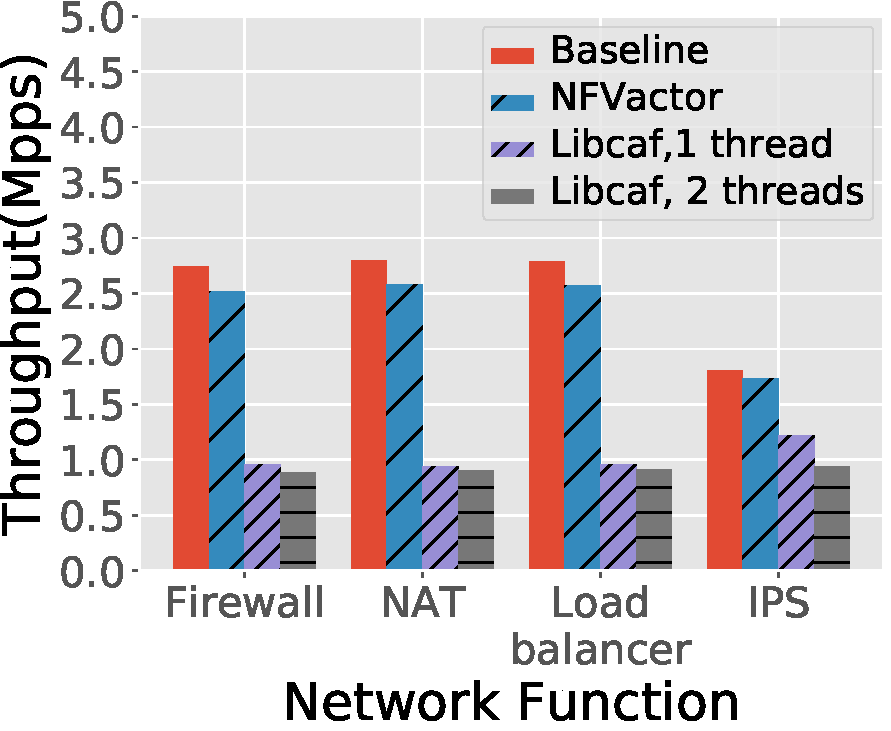
\includegraphics[width=\columnwidth]{chap-nfvactor/exp-figure/micro_throughput.pdf}
    \caption{}\label{fig:micro_throughput}
  \end{subfigure}\hfill
  \begin{subfigure}[t]{0.49\linewidth}
    \centering
    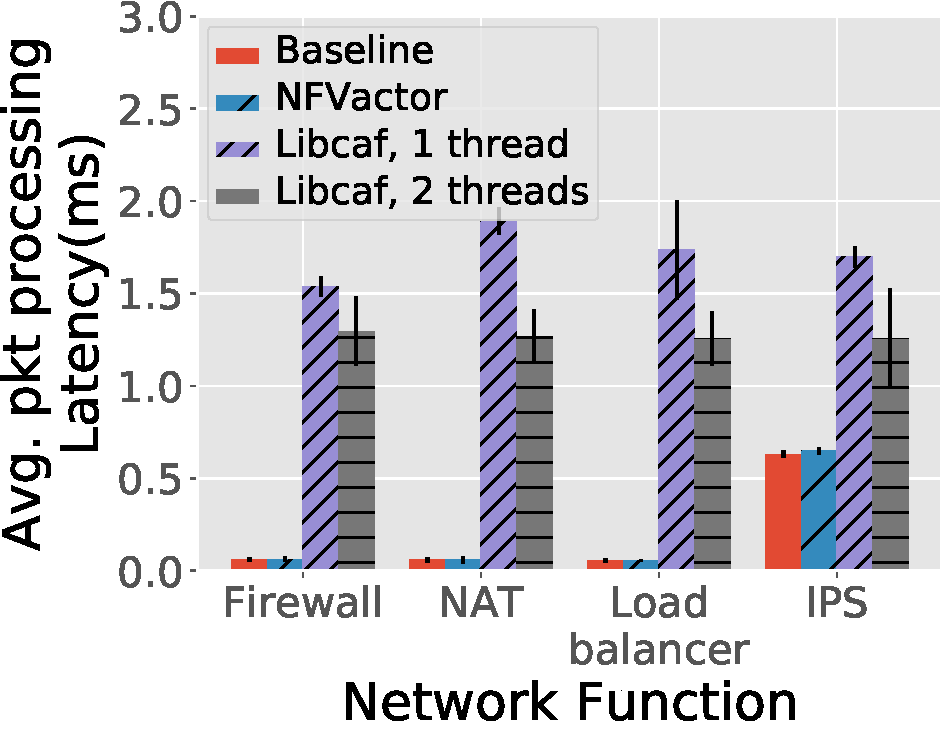
\includegraphics[width=\columnwidth]{chap-nfvactor/exp-figure/micro_latency.pdf}
    \caption{}\label{fig:micro_latency}
  \end{subfigure}\hfill
  \begin{subfigure}[t]{0.49\linewidth}
    \centering
    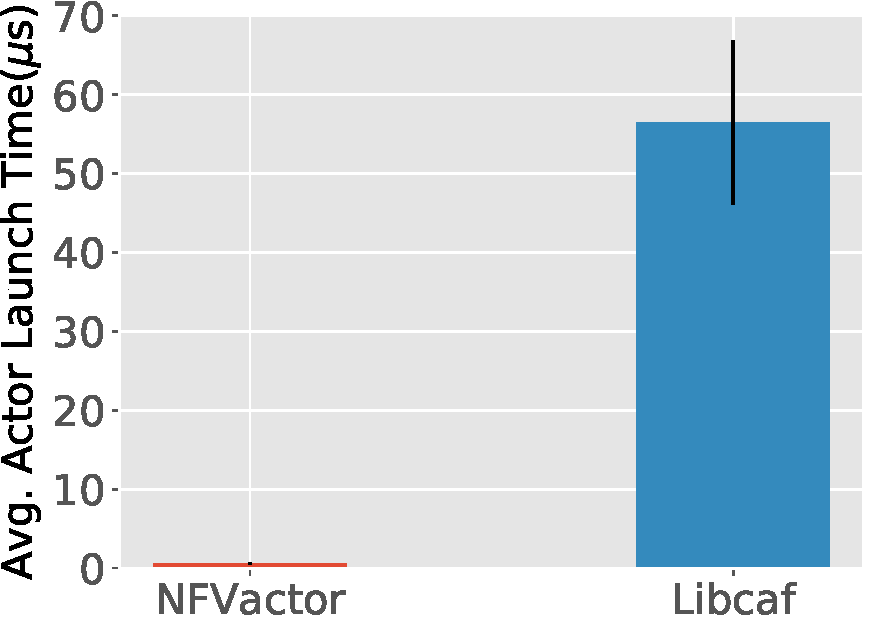
\includegraphics[width=\columnwidth]{chap-nfvactor/exp-figure/micro_launch_time.pdf}
    \caption{}\label{fig:micro_launch_time}
  \end{subfigure}\hfill
  \begin{subfigure}[t]{0.49\linewidth}
    \centering
    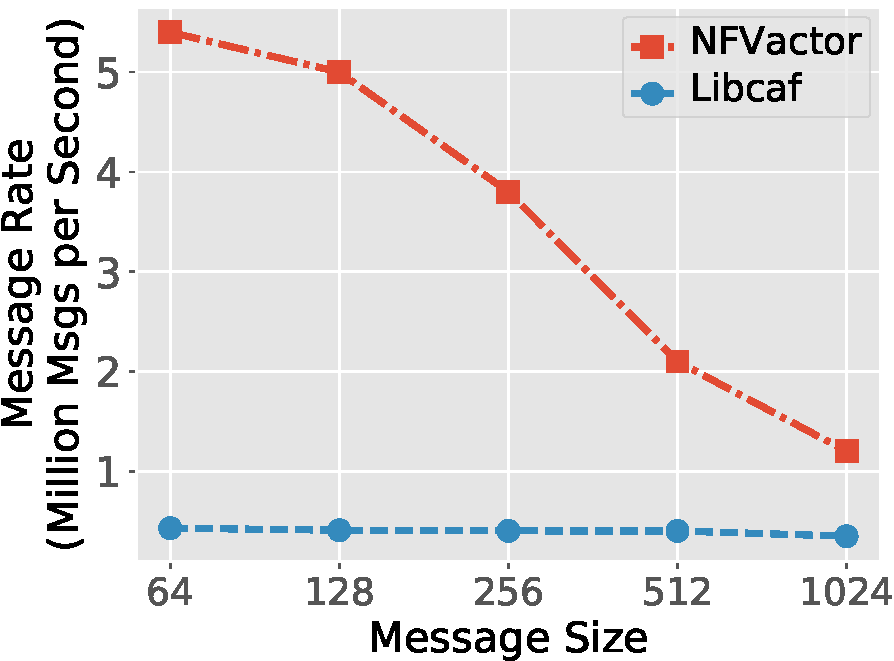
\includegraphics[width=\columnwidth]{chap-nfvactor/exp-figure/micro_mp.pdf}
    \caption{}\label{fig:micro_mp}
  \end{subfigure}
\caption{Performance of the Runtime.}
\end{figure}

\subsubsection{Packet processing throughput and latency}
\label{sec:packet-processing-tl}

We first evaluate the packet processing throughput (number of packets processed per second) and latency (difference between the time that a packet enters the runtime to the time this packet is released from the runtime) of the \nfactor~runtime by running the four implemented NFs. The traffic generator produces flows with 64-byte TCP packets, a 10pps (packets per second) flow rate and a 10-second active time. The overall packet rate of the input traffic is 5Mpps. For comparison, we also evaluate performance of libcaf runtime. We vary the number of worker threads used by the libcaf runtime to reflect the performance overhead of thread synchronization. Finally, we compare with four baseline NFs. The baseline NFs are implemented using a normal packet processing loop, sharing similar processing logic as the $process\_pkt$ API. The per-flow state in each baseline NF is stored in a fast hash table \cite{pagh2001cuckoo} without using the actor abstraction.

Fig.~\ref{fig:micro_throughput} and Fig.~\ref{fig:micro_latency} show that \nfactor~runtime achieves significantly larger throughput and smaller processing latency than libcaf runtime, and the performance of the NFs in~\nfactor~is close to that of the baseline NFs, as the actor abstraction does introduce a small overhead. According to Fig.~\ref{fig:micro_throughput}, when the number of the worker threads used by libcaf is increased, the total throughput drops by a small margin, due to increased synchronization overhead between the polling thread and multiple worker threads.



\subsubsection{Actor launch time and sending rate of remote actor messages}
\label{sec:srram}

The actor launch time is the time when the first packet of a flow is received to the time when this packet is processed by the launched actor. It is a strong performance indicator of the actor runtime system. In Fig.~\ref{fig:micro_launch_time}, the input traffic is the same as in Sec.~\ref{sec:packet-processing-tl}. We see that the average actor launch time in \nfactor~is much smaller than that of the libcaf runtime, as \nfactor~pre-allocates flow actors into a ring buffer to speed-up actor launch time.

Fig.~\ref{fig:micro_mp} shows the average sending rate of remote actor messages between two runtimes running on different servers. For various message sizes, the message rate achieved by~\nfactor~is significantly larger than that of libcaf. Especially, when the message size is larger than 256 bytes, we measure the consumed bandwidth of~\nfactor~to be around 9.1Gbps, which is close to the 10Gbps line rate. This result reflects that our user-space message passing module can significantly improve the performance of remote actor communication.

%When the size of each remote actor message is smaller than 128 bytes, the message rate is limited by about 5M messages (the worker thread's limitation decided by the CPU frequency), and the line speed is not reached; when the size of each remote actor message is larger than 256 bytes, the worker thread only needs to send out a smaller number of messages while saturating the line speed. In contrast, with libcaf, the messaging rate is limited by the bottleneck of enqueuing and dequeuing messages to a broker thread \cite{caf}, and the line speed cannot be approached.

\subsection{System Scalability}
\label{sec:ppt}

\begin{figure}[!h]
  \begin{subfigure}[t]{0.49\linewidth}
    \centering
    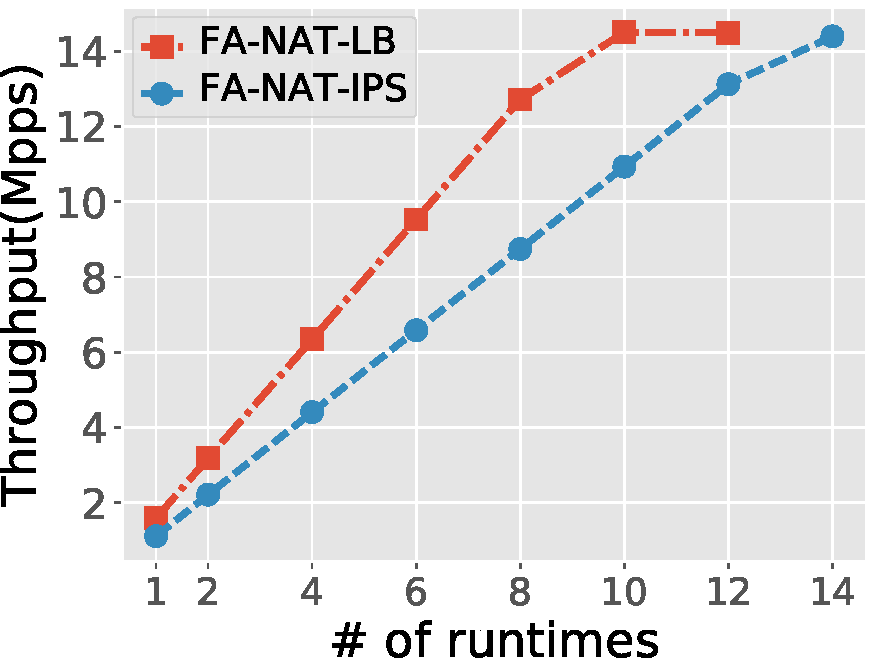
\includegraphics[width=\columnwidth]{chap-nfvactor/exp-figure/throughput_scaling.pdf}
    \caption{}\label{fig:throughput_scaling}
  \end{subfigure}\hfill
  \begin{subfigure}[t]{0.49\linewidth}
   \centering
   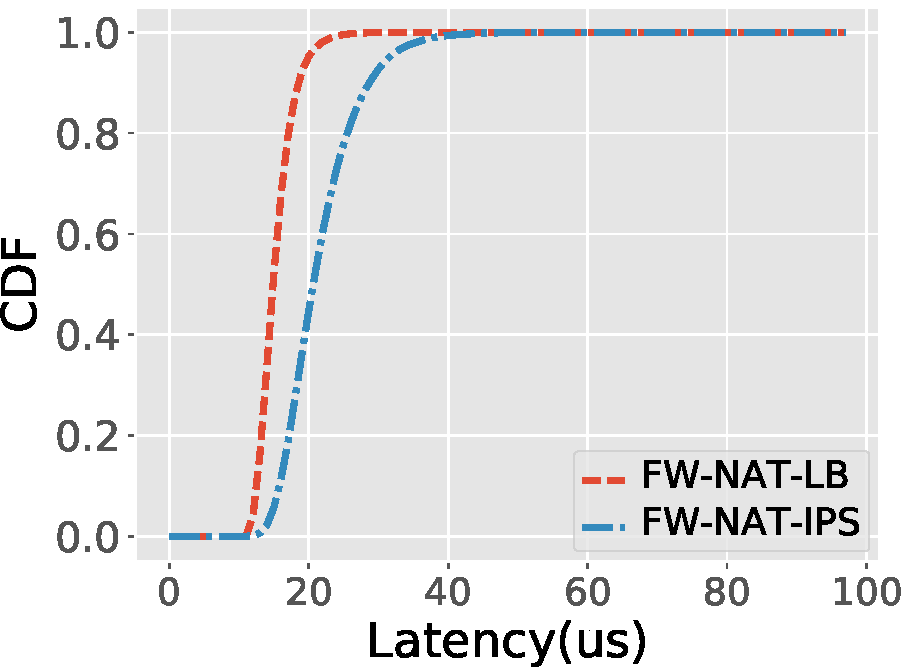
\includegraphics[width=\columnwidth]{chap-nfvactor/exp-figure/throughput_latency_cdf.pdf}
   \caption{}\label{fig:throughput_latency_cdf}
  \end{subfigure}\hfill
  \begin{subfigure}[t]{0.49\linewidth}
   \centering
   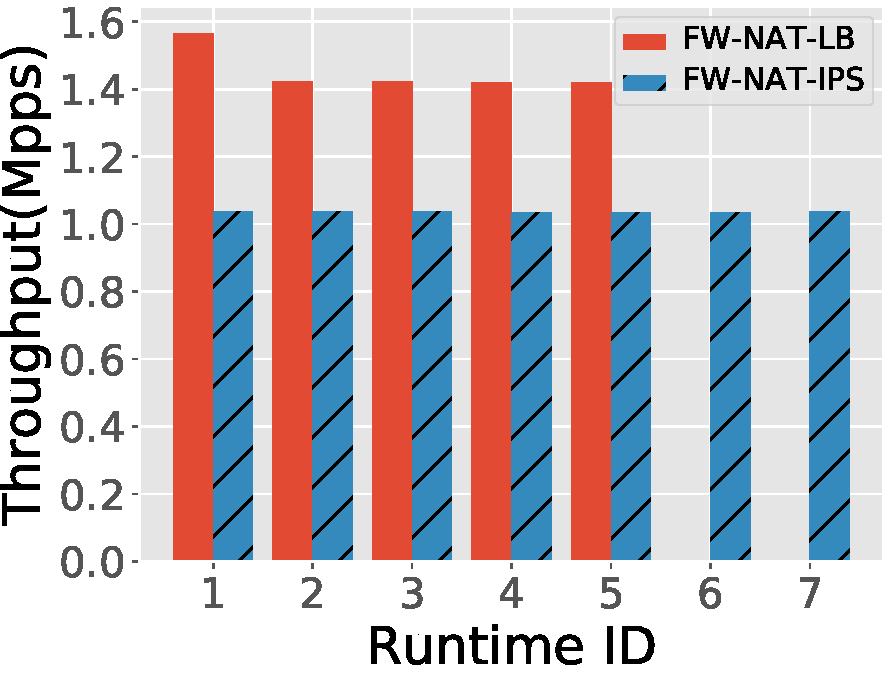
\includegraphics[width=\columnwidth]{chap-nfvactor/exp-figure/throughput_2sc.pdf}
   \caption{}\label{fig:throughput_2sc}
  \end{subfigure}
  \begin{subfigure}[t]{0.49\linewidth}
    \centering
    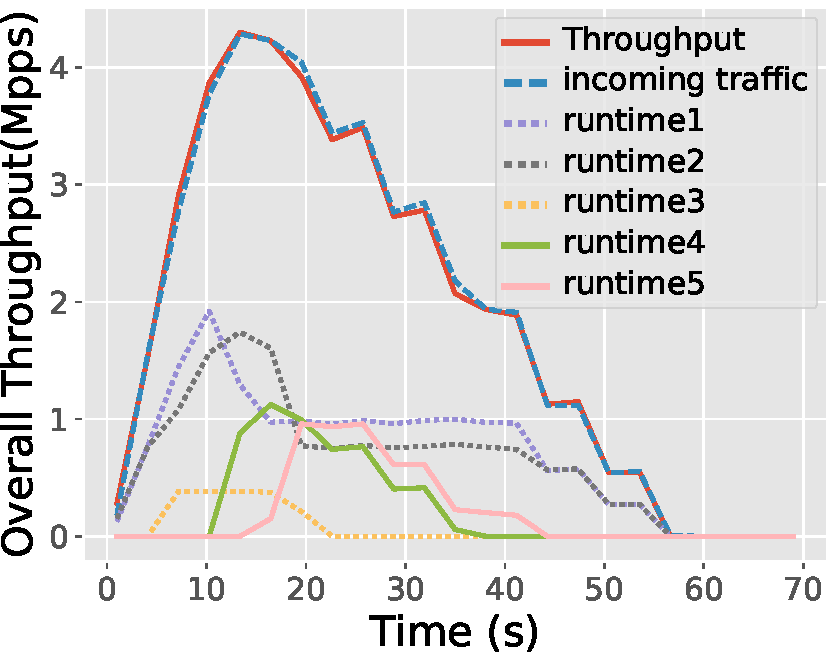
\includegraphics[width=\columnwidth]{chap-nfvactor/figure/Scale.pdf}
    \caption{Dynamic scaling.}\label{fig:scale}
  \end{subfigure}\hfill
\caption{System scalability.}
\end{figure}

We now evaluate the maximum packet processing throughput of \nfactor~as the number of runtimes increases. We use two servers and configure the runtimes with service chain `firewall (FW) $\rightarrow$ NAT $\rightarrow$ load balancer (LB)' (in one set of experiments) or service chain `firewall (FW) $\rightarrow$ NAT $\rightarrow$ IDS' (in another set of experiments). To fully stress the system, we configure traffic generators to produce a mixture of short flows and long flows up to 10Gbps line rate. A short flow consists of 64-byte TCP packets with a 10pps packet rate and lasts for 1 second. A long flow consists of 64-byte TCP packets with a 10pps packet rate and lasts for 10 seconds. Each type of flow consumes half of generated bandwidth. We gradually increase the number of active runtimes and collect the total throughput achieved by the runtimes.

Fig.~\ref{fig:throughput_scaling} shows the overall packet processing throughput increases linearly with the increase of the runtimes. Overall throughput of 14.49Mpps (9.70Gbps) and 14.39Mpps (9.67Gbps) are achieved when the runtimes run service chain `FW $\rightarrow$ NAT $\rightarrow$ LB'and `FW $\rightarrow$ NAT $\rightarrow$ IDS', respectively.
This verifies that~\nfactor~can approach 10Gbps line-rate packet processing for 64-byte small packets, even when the input traffic consists of many short-lived flows. %We believe that~\nfactor~can handle 10Gbps line-rate with fewer runtimes if the input traffic has less short-lived flows.

Fig.~\ref{fig:throughput_latency_cdf} shows the CDF of packet processing latencies, collected during a 20s period when 10 and 14 runtimes are used to run `FW $\rightarrow$ NAT $\rightarrow$ LB' and `FW $\rightarrow$ NAT $\rightarrow$ IDS', respectively. The average latency for both service chain is around 20$\mu$s.

We next run the two service chains concurrently in the system. We run 5 runtimes in one server configured with `FW $\rightarrow$ NAT $\rightarrow$ LB' and 7 runtimes in another server configured with `FW $\rightarrow$ NAT $\rightarrow$ IDS'. The input traffic has a total packet rate of 14.50Mpps and shares the same mixed pattern to produce Fig.~\ref{fig:throughput_scaling}. The input traffic is evenly split among the two service chains. Fig.~\ref{fig:throughput_2sc} shows the throughput of each runtime. We can see that a total throughput of 7.25Mpps can be reached by each service chain. The workload is also evenly balanced among runtimes in the same server, demonstrating the effectiveness of our virtual switches for load balancing under mixed short and long flows.

Finally, the performance of the dynamic scaling controlled by the coordinator is shown in Fig.~\ref{fig:scale}. The traffic generator generates traffic with increasing packet rate for the first 15 seconds, and then gradually decreases the packet rate of the traffic for the last 45 seconds. %A total number of 100K flows is generated throughout the experiment.
The cluster is initialized with two runtimes (runtime 1 and 2) running `FW $\rightarrow$ NAT $\rightarrow$ IDS' service chain. Starting from the 10th second, runtimes 1 and 2 become overloaded and their workload is gradually migrated away to runtime 4 and 5. With dynamic scaling, the achieved throughput can correctly match the input traffic during the 60 seconds.

\subsection{Performance of Flow Replication}
\label{sec:rp}

\begin{figure}[!h]
 \begin{subfigure}[t]{0.49\linewidth}
		\centering
		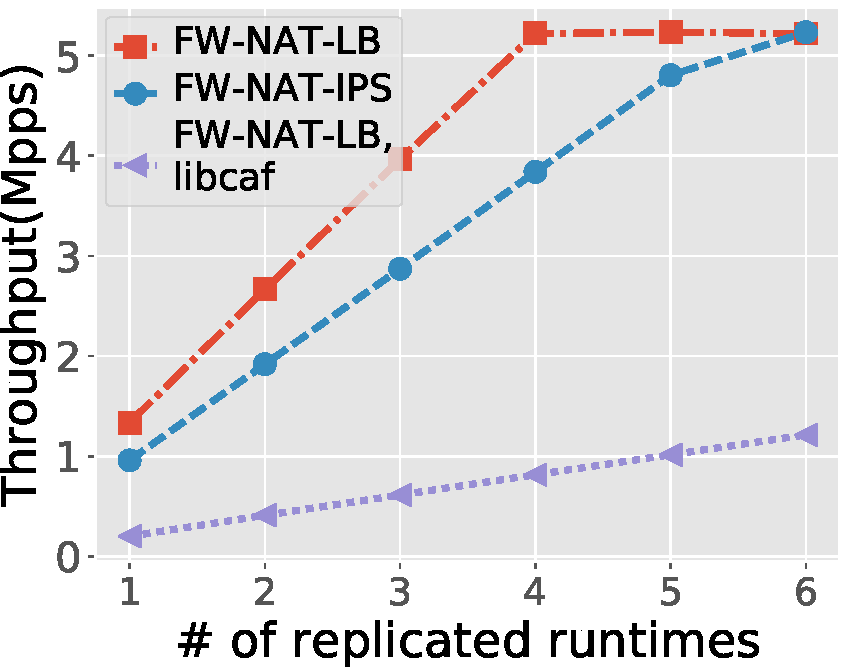
\includegraphics[width=\columnwidth]{chap-nfvactor/exp-figure/rep_scaling.pdf}
		\caption{}\label{fig:rep_scaling}
	 \end{subfigure}\hfill
	 \begin{subfigure}[t]{0.49\linewidth}
	\centering
		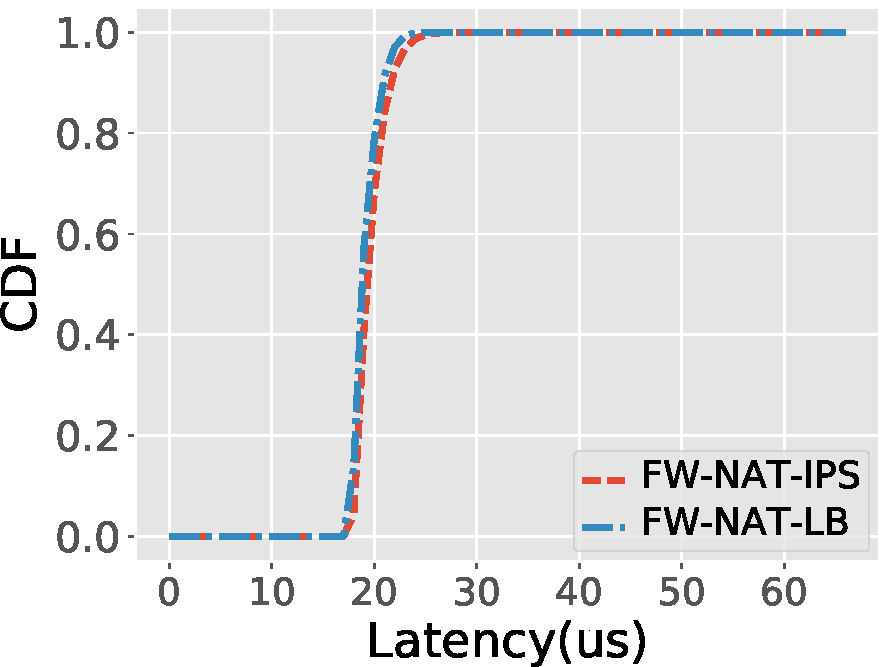
\includegraphics[width=\columnwidth]{chap-nfvactor/exp-figure/rep_latency_pdf.pdf}
		\caption{}\label{fig:rep_latency_pdf} \end{subfigure}
	\caption{Performance of flow replication.}
\label{fig:rep-perf}
\end{figure}

\begin{table}[!h]
\centering
\caption{Recovery time and \# of flows recovered}
\vspace{-3mm}
\label{table:recover}
\resizebox{\columnwidth}{!}{
\begin{tabular}{|l|l|l|l|}
\hline
                                                                                   & FW$\rightarrow$NAT$\rightarrow$LB          & FW$\rightarrow$NAT$\rightarrow$IDS            & FW$\rightarrow$NAT$\rightarrow$LB, libcaf           \\ \hline
\begin{tabular}[c]{@{}l@{}}Average recovery time\\ for each runtime\end{tabular}   & 65.3ms             & 66.6ms             & 934.2ms           \\ \hline
\begin{tabular}[c]{@{}l@{}}Number of flows recovered\\ on each runtime\end{tabular} & at least 87k flows & at least 87k flows & at least 20k flows \\ \hline
\end{tabular}
}
\vspace{-3mm}
\end{table}

In this set of experiments, input flows are produced following the same mixed pattern to produce Fig.~\ref{fig:throughput_scaling}. The coordinator chooses two servers and launches the same number of runtimes on them. The coordinator instructs each runtime on a server to replicate its flows to a distinct runtime in another server. We gradually increase packet rate of the input traffic and the number of runtimes running on each server, to investigate throughput and scalability when flow replication is enabled.

Fig.~\ref{fig:rep_scaling} shows that both service chains can scale up to handle the 5.22Mpps input packet rate when six runtimes running on a server concurrently replicate their traffic to six replica runtimes on another server. In particular, when the input rate reaches 5.22Mpps, the measured bandwidth on the link for transmitting replication messages reaches almost 10Gbps. When the libcaf version of implementation is used, the replication throughput is significantly lower.

Fig.~\ref{fig:rep_latency_pdf} shows the CDF of packet processing latencies of \nfactor~when flow replication is enabled. The latency measured in this experiment is difference between the time that the packet enters replication source runtime to the time this packet is released from the replication target runtime. For both service chains, the number of runtimes on each of the two servers is 6 while the input packet rate is 5.22Mpps. The average latency is around 20$\mu$s for both service chains.

Table \ref{table:recover} shows the average recovery time of 6 replication target runtimes when their corresponding replication source runtimes fail simultaneously. We can see that \nfactor~has a much shorter recovery time than the libcaf version even when processing a larger number of flows.

\vspace{-3mm}
\subsubsection{Comparison with FTMB} We compare the performance of flow replication in \nfactor~with the reported performance of FTMB \cite{sherry2015rollback}. Both systems achieve throughput up to millions of packets per second and recovery time of tens of milliseconds with flow replication enabled. \nfactor~has a more stable packet processing latency (according to Fig.~\ref{fig:rep_latency_pdf}, smaller than 70 microseconds, with an average of 20 microseconds) because it does not need to checkpoint the runtime, whereas FTMB introduces a relatively high packet processing latency (up to 3000 microseconds) when checkpointing kicks in.

\subsection{Performance of Flow Migration}
\label{sec:fmp}

\begin{figure}[!h]
 \begin{subfigure}[t]{0.49\linewidth}
   \centering
   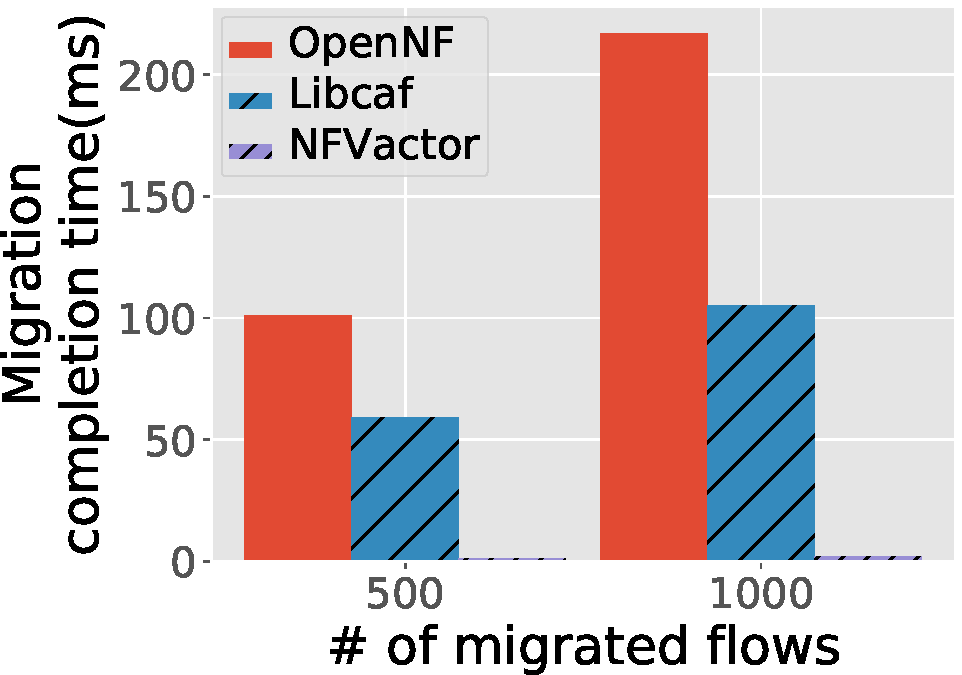
\includegraphics[width=\columnwidth]{chap-nfvactor/exp-figure/migration_compare.pdf}
   \caption{}\label{fig:migration_compare} \end{subfigure}\hfill
  \begin{subfigure}[t]{0.49\linewidth}
   \centering
   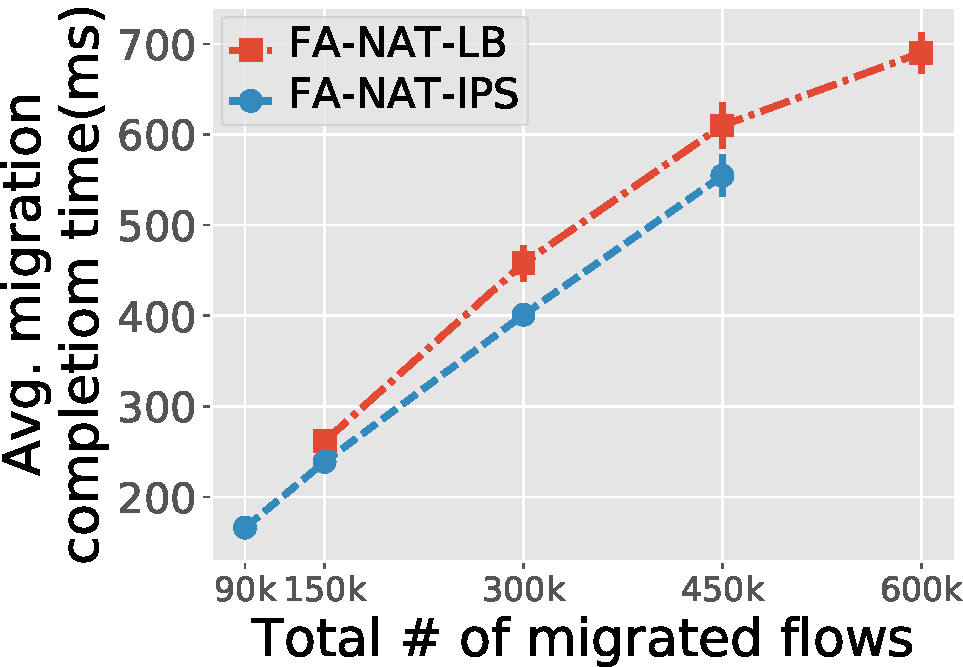
\includegraphics[width=\columnwidth]{chap-nfvactor/exp-figure/migration_time.pdf}
   \caption{}\label{fig:migration_time}
  \end{subfigure}
\caption{Flow migration completion time.}
\end{figure}

We first compare flow migration performance among \nfactor, libcaf runtime, and OpenNF. Both \nfactor~and libcaf runtime run the example firewall. We also port the example firewall to work with OpenNF. We send the same number of flows to the three firewalls and each flow has a 10pps packet rate. In Fig.~\ref{fig:migration_compare}, the time to migrate the respective number of flows is much smaller with \nfactor~(0.7ms for 500 flows and 1.5ms for 1000 flows), when compared to OpenNF (101ms for 500 flows and 217ms for 1000 flows) and the libcaf runtime (59ms for 500 flows and 105ms for 1000 flows). Due to efficient runtime design, \nfactor~can out-perform OpenNF by 144 times when migrating 1000 flows.

%To inspect performance of flow migration in \nfactor,
We next show the time taken for concurrently migrating a large number of flows among multiple pairs of runtimes. The traffic generator produces a number of flows with a 10pps flow rate, each lasting for 1 minute. The flows are first sent to three runtimes running in one server. Then the coordinator instructs the three runtimes to concurrently migrate all the flows to three runtimes running in another server. %This experiment tests the same service chain configurations as in Sec.~\ref{sec:ppt} and the number of flows injected to each runtime is varied.

Fig.~\ref{fig:migration_time} shows the average migration completion time of the three migration source runtimes. The standard deviation of the completion time is shown as error bar in Fig.~\ref{fig:migration_time} as well. \nfactor~can migrate 600K flows (with 6Mpps total throughput) from three migration source runtimes running in one server to three migration target runtimes running in another server using around 700ms. Besides the performance boost enabled by efficient runtime design, the decentralized flow migration also contributes to the performance. Since the flow migration are concurrently carried out among three pairs of runtimes, each pair of runtime only needs migrates around 200K flows. This significantly reduce the eventual flow migration completion time for all the 600K flows. If the 600K flows are sequentially migrated, the resulted flow migration completion time may be prolonged to over 2 seconds. Finally, throughout the evaluation in Fig.~\ref{fig:migration_time}, we observe zero packet loss caused by our flow migration protocol.
%All these factors verify the effectiveness and robustness of our decentralized flow migration design.

% it takes 400-500ms to migrate 100k flows (with 1Mpps total throughput) on a single runtime, making flow migration a practical approach to resolve hot spots. Considering flow migration is concurrently carried out between three pairs of runtimes, it also demonstrates efficiency of our distributed flow migration protocol. In our experiments, we also observe no packet loss is caused by flow migration, validating the loss-avoidance property.

\begin{comment}
\subsection{Other Applications}
\label{sec:applications}

\begin{figure}[!h]
  \begin{subfigure}[t]{0.49\linewidth}
   \centering
   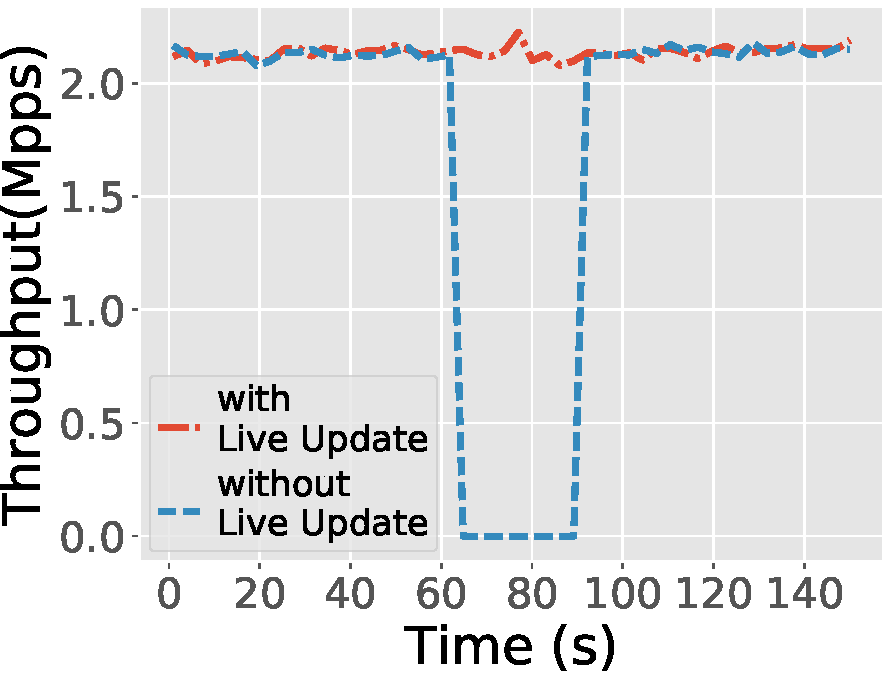
\includegraphics[width=\columnwidth]{figure/Dynamic.pdf}
   \caption{Live NF update.}\label{fig:dynamic}
  \end{subfigure}\hfill
  \begin{subfigure}[t]{0.49\linewidth}
   \centering
   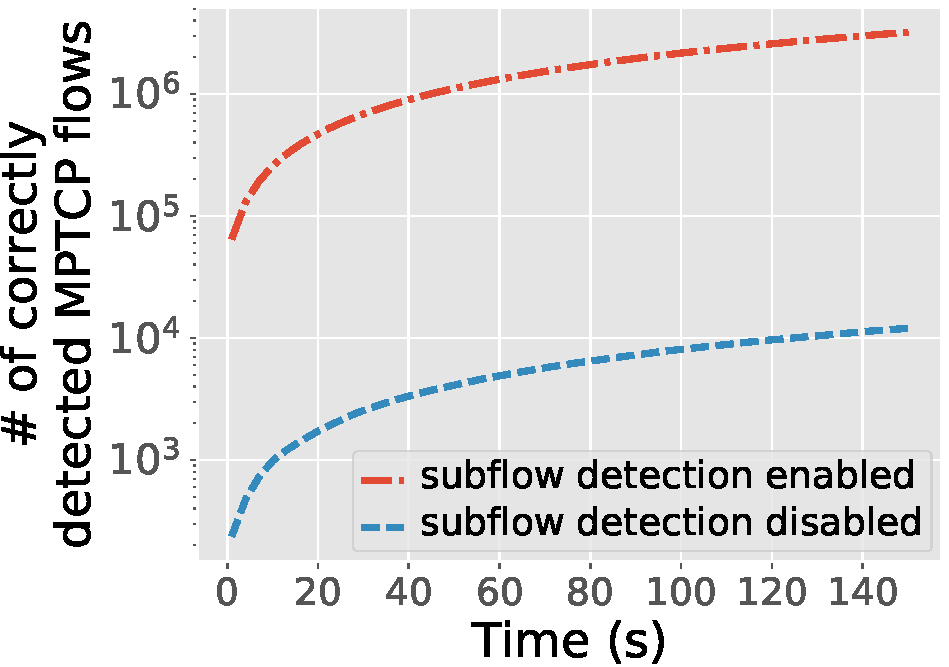
\includegraphics[width=\columnwidth]{figure/Mptcp.pdf}
   \caption{MPTCP subflow detection.}\label{fig:mptcp}
  \end{subfigure}
  \vspace{-2mm}
\caption{Other applications.}
\vspace{-4mm}
\end{figure}

In addition, we build two applications based on \nfactor, which exploit its lightweight, distributed flow migration capability to achieve useful functionalities.

\vspace{1mm}
\noindent\textbf{Live NF update.} \nfactor~can achieve dynamic NF update (\eg, software version, important NF configuration files) without interfering with active flows, by dynamically migrating the flows out to a replica runtime, performing update and migrating the flows back. Fig.~\ref{fig:dynamic} illustrates the throughput of a runtime running a firewall NF, during dynamic update of its firewall rule. No active flows are dropped during the update with \nfactor, while significant throughput drop occurs if shutting down the firewall for its update.

\vspace{1mm}
\noindent\textbf{MPTCP sub-flow processing.} When an MPTCP \cite{wischik2011design} flow traverses an NFV system, its sub-flows may be sent to different NF instances for processing. However, some NFs require all subflows to be processed by the same instance, \eg, IDS \cite{snort}. In \nfactor, we create a new NF for MPTCP sub-flows detection. Whenever the flow actor processes the first packet of a flow with this NF, the NF checks whether it belongs to an MPTCP flow. If so, the NF performs a consistent hashing using the MPTCP header to decide a migration target runtime in the cluster, and notify the flow actor to migrate itself to the target. In this way, different sub-flows belonging to the same MPTCP flow can be processed by the same flow actor. In existing flow migration systems, it is hard to incorporate sub-flow detection directly into the NFs: the NFs lack per-flow execution environment as in~\nfactor~and they can not initiate flow migration by themselves without instructions from the centralized controller.

In the experiment of Fig.~\ref{fig:mptcp}, we inject a total number of about 3.2M MPTCP flows to 3 runtimes. With subflow detection enabled, the total number of correctly processed MPTCP flows, \ie, those whose subflows are all processed by the same runtime, is always the same as the total number of input MPTCP flows. Without this detection, most of the subflows are processed by different runtimes.
\end{comment}
